% PRL flow chart: second-order pipeline (SS by complex-r quadrature; SR by the hybrid split).
% Two-column width (17.8 cm). Compile with pdflatex.
\documentclass[tikz,border=2pt]{standalone}
\usepackage[T1]{fontenc}
\usepackage{lmodern}
\usepackage{amsmath,amssymb}
\usetikzlibrary{arrows.meta,decorations.pathreplacing,calc}
\newcommand{\PP}{\Phi^{\rm P}}
\newcommand{\Pres}{\Phi^{\rm res}}
\begin{document}
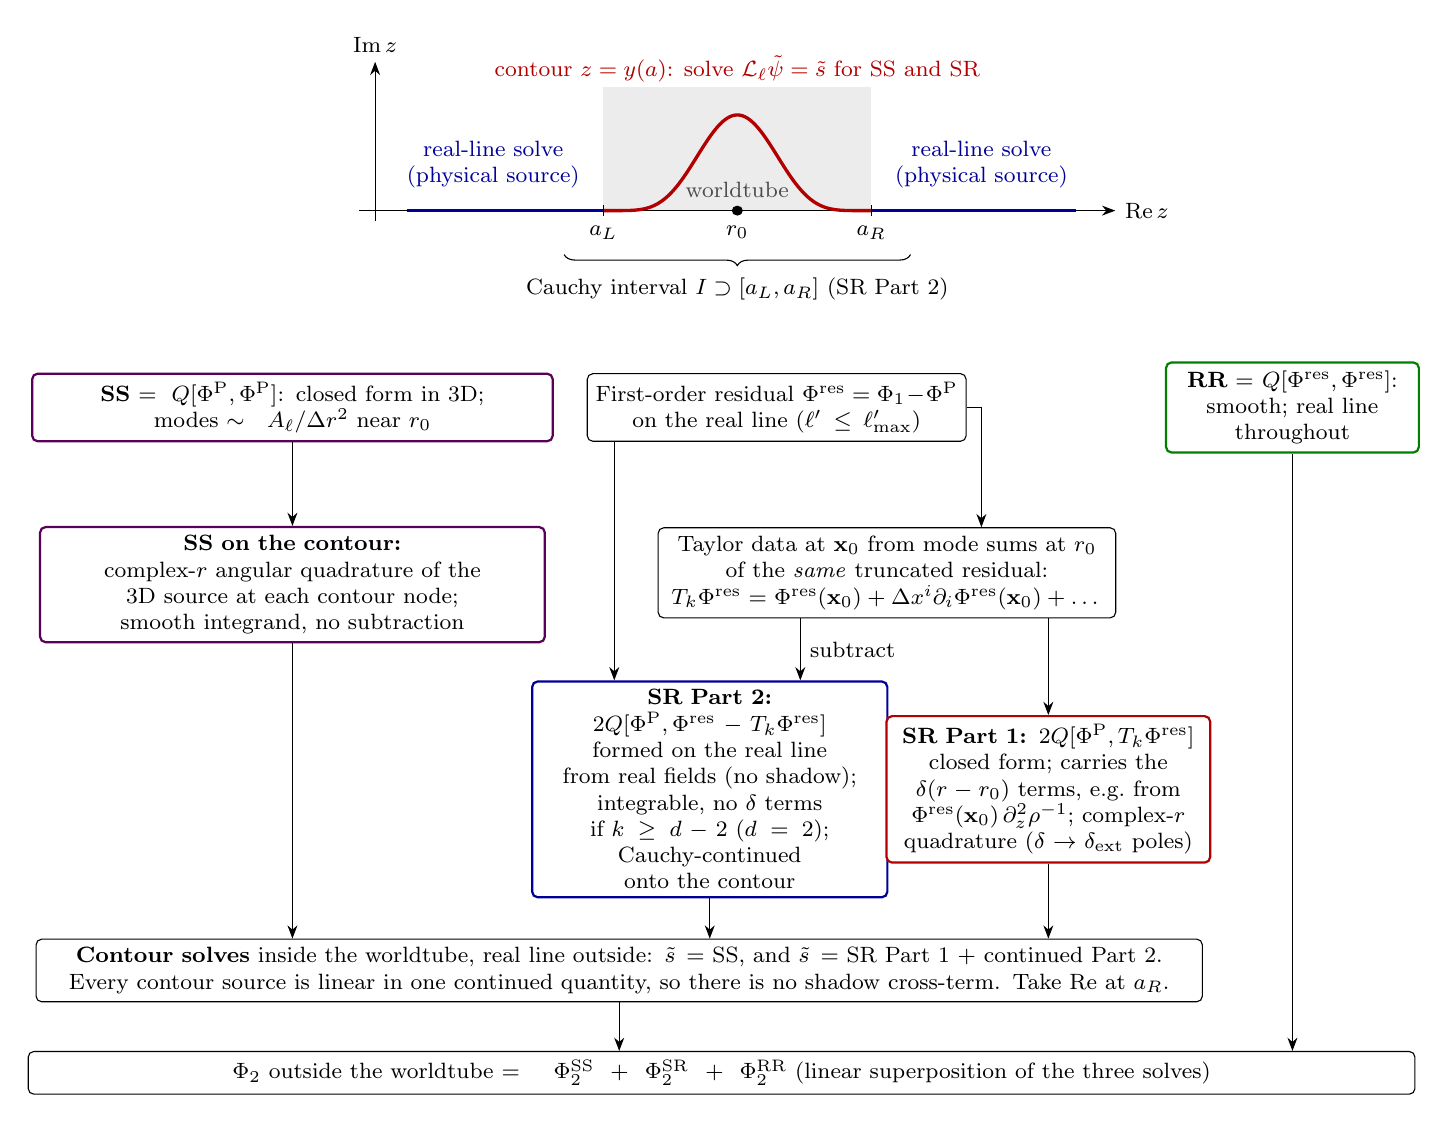
\begin{tikzpicture}[>=Stealth, font=\footnotesize,
  box/.style={draw, rounded corners=2pt, align=center, inner sep=3pt, text width=#1, fill=white},
  box/.default=4cm]

% ---------- complex r-plane ----------
\begin{scope}[xshift=4.1cm, yscale=0.9]
\fill[gray!15] (3.3,0) rectangle (6.7,1.75);
\node[gray!60!black] at (5,0.3) {worldtube};
\draw[->] (0.2,0) -- (9.8,0) node[right] {$\operatorname{Re} z$};
\draw[->] (0.4,-0.15) -- (0.4,2.1) node[above] {$\operatorname{Im} z$};
\draw[very thick, blue!60!black] (0.8,0) -- (3.3,0);
\draw[very thick, blue!60!black] (6.7,0) -- (9.3,0);
\draw[very thick, red!70!black, domain=3.3:6.7, samples=120, smooth]
  plot (\x, {1.35*(1-((\x-5)/1.7)^2)^6});
\fill (5,0) circle (2pt);
\node[below=2pt] at (5,0) {$r_0$};
\draw (3.3,0.08) -- (3.3,-0.08) node[below] {$a_L$};
\draw (6.7,0.08) -- (6.7,-0.08) node[below] {$a_R$};
\draw[decorate, decoration={brace, mirror, amplitude=4pt}]
  (2.8,-0.62) -- (7.2,-0.62) node[midway, below=5pt]
  {Cauchy interval $I\supset[a_L,a_R]$ (SR Part 2)};
\node[blue!60!black, align=center] at (1.9,0.65) {real-line solve\\(physical source)};
\node[blue!60!black, align=center] at (8.1,0.65) {real-line solve\\(physical source)};
\node[red!70!black] at (5,2.0) {contour $z=y(a)$: solve $\mathcal L_\ell\tilde\psi=\tilde s$ for SS and SR};
\end{scope}

% ---------- row 1: the three pieces ----------
\node[box=6.4cm, draw=violet!70!black, thick] (ss) at (3.45,-2.5)
  {\textbf{SS} $=Q[\PP,\PP]$: closed form in 3D;\\modes $\sim A_\ell/\Delta r^2$ near $r_0$};
\node[box=4.6cm] (res) at (9.6,-2.5)
  {First-order residual $\Pres=\Phi_1-\PP$\\on the real line ($\ell'\le\ell'_{\max}$)};
\node[box=3.0cm, draw=green!50!black, thick] (rr) at (16.15,-2.5)
  {\textbf{RR} $=Q[\Pres,\Pres]$:\\smooth; real line\\throughout};

% ---------- row 2: SS quadrature and Taylor data ----------
\node[box=6.2cm, draw=violet!70!black, thick] (ss1) at (3.45,-4.75)
  {\textbf{SS on the contour:}\\complex-$r$ angular quadrature of the\\3D source at each contour node;\\smooth integrand, no subtraction};
\node[box=5.6cm] (tay) at (11.0,-4.6)
  {Taylor data at $\mathbf x_0$ from mode sums at $r_0$\\of the \emph{same} truncated residual:\\$T_k\Pres=\Pres(\mathbf x_0)+\Delta x^i\partial_i\Pres(\mathbf x_0)+\dots$};

% ---------- row 3: SR split ----------
\node[box=4.3cm, draw=blue!60!black, thick] (sr2) at (8.75,-7.35)
  {\textbf{SR Part 2:} $2Q[\PP,\Pres-T_k\Pres]$\\formed on the real line\\from real fields (no shadow);\\integrable, no $\delta$ terms\\if $k\ge d-2$ ($d=2$);\\Cauchy-continued\\onto the contour};
\node[box=3.9cm, draw=red!70!black, thick] (sr1) at (13.05,-7.35)
  {\textbf{SR Part 1:} $2Q[\PP,T_k\Pres]$\\closed form; carries the\\$\delta(r-r_0)$ terms, e.g.\ from\\$\Pres(\mathbf x_0)\,\partial_z^2\rho^{-1}$; complex-$r$\\quadrature ($\delta\to\delta_{\rm ext}$ poles)};

% ---------- rows 4–5 ----------
\node[box=14.6cm] (con) at (7.6,-9.65)
  {\textbf{Contour solves} inside the worldtube, real line outside: $\tilde s=$ SS, and $\tilde s=$ SR Part 1 $+$ continued Part 2.\\Every contour source is linear in one continued quantity, so there is no shadow cross-term. Take $\operatorname{Re}$ at $a_R$.};
\node[box=17.4cm] (out) at (8.9,-10.95)
  {$\Phi_2$ outside the worldtube $=\Phi_2^{\rm SS}+\Phi_2^{\rm SR}+\Phi_2^{\rm RR}$ (linear superposition of the three solves)};

% ---------- arrows ----------
\draw[->] (ss.south -| ss1) -- (ss1.north);
\draw[->] (res.east) -| ($(tay.north)+(1.2,0)$);
\draw[->] ($(res.south west)+(0.35,0)$) -- ({$(res.south west)+(0.35,0)$} |- sr2.north);
\draw[->] (tay.south -| sr1) -- (sr1.north);
\draw[->] (tay.south -| 9.9,0) -- node[right] {subtract} (9.9,0 |- sr2.north);
\draw[->] (ss1.south) -- (ss1.south |- con.north);
\draw[->] (sr2.south) -- (sr2.south |- con.north);
\draw[->] (sr1.south) -- (sr1.south |- con.north);
\draw[->] (rr.south) -- (rr.south |- out.north);
\draw[->] (con) -- (con |- out.north);
\end{tikzpicture}
\end{document}
